\Needspace{10\baselineskip}
\subsection{Quy trình đặt chỗ và thanh toán}
\label{sec:execution-booking-payment}

Quy trình bắt đầu khi người thuê đã đăng nhập và lựa chọn một không gian đang được công bố. Phòng có một hình thức thuê đang hoạt động: theo giờ hoặc theo tháng/quý. Người thuê chọn thời gian theo hình thức đó, không tự chuyển loại thuê của phòng. Trong phiên bản hiện tại, bước thanh toán QR được áp dụng cho phòng thuộc Host demo đã cấu hình kênh payOS.

\Needspace{7\baselineskip}
\subsubsection{Lựa chọn không gian và kiểm tra thời gian thuê}
Người thuê thực hiện các bước sau trước khi mở phiên thanh toán:
\begin{enumerate}
\item Từ danh sách hoặc bản đồ, mở chi tiết phòng để xem ảnh, địa chỉ, tiện ích, giá và điều kiện sử dụng, sau đó chọn đặt chỗ.
\item Chọn ngày và khung giờ nếu thuê theo giờ; chọn kỳ một hoặc ba tháng nếu thuê cố định. Màn hình đọc lịch để thể hiện khoảng đã thuê hoặc đang giữ tạm.
\item Thực hiện kiểm tra lịch và giá. Hệ thống đối chiếu lịch hoạt động, khoảng khóa và các booking đang giữ chỗ, rồi hiển thị tiền thuê cùng khoản trả trước 40\% như Hình~\ref{fig:booking-quote-qr}.
\end{enumerate}

Kết quả kiểm tra không thay cho việc giữ lịch. Khi người thuê nhấn thanh toán, transaction đọc lại dữ liệu và tạo booking PENDING cùng phần giữ lịch tạm. Yêu cầu vừa bị người khác đặt trùng phải được kiểm tra lại; việc gửi lại cùng yêu cầu không được tạo thêm một lượt thuê độc lập. Booking lưu giá và thời gian đã chốt để tiếp tục bước thanh toán.

\subsubsection{Thanh toán QR và xác nhận đặt chỗ}
Sau khi tạo booking, ứng dụng gọi backend Java để lấy giao dịch payOS và chuyển thẳng tới màn QR. Backend xác minh ID token, người thuê của booking và Host thuộc kênh demo; số tiền được lấy từ snapshot, không nhận giá do client tự khai báo. Hạn phiên là mốc đến trước giữa thời điểm tạo booking cộng năm phút và giờ bắt đầu thuê. Việc mở lại QR không làm tính lại thời hạn từ đầu.

\IfFileExists{Resources/chapter6/booking-qr.png}{%
\begin{figure}[H]
\begin{minipage}{\linewidth}
\setlength{\parindent}{1.27cm}
\setstretch{1.4}
Trong Hình~\ref{fig:booking-quote-qr}(a), lượt thuê một giờ có giá 5.000 đồng và khoản trả trước 2.000 đồng. Sau khi gửi yêu cầu, màn QR ở Hình~\ref{fig:booking-quote-qr}(b) hiển thị đúng khoản tiền này, mã giao dịch, người nhận và thời gian còn lại. Người thuê chuyển khoản theo QR hoặc mở trang payOS. Nếu rời màn hình, thẻ tiếp tục thanh toán và thông báo điện thoại dẫn về đúng giao dịch còn hạn; thời gian giữ lịch không bắt đầu lại.
\par\medskip
\centering
\begin{minipage}[t]{0.40\linewidth}\centering
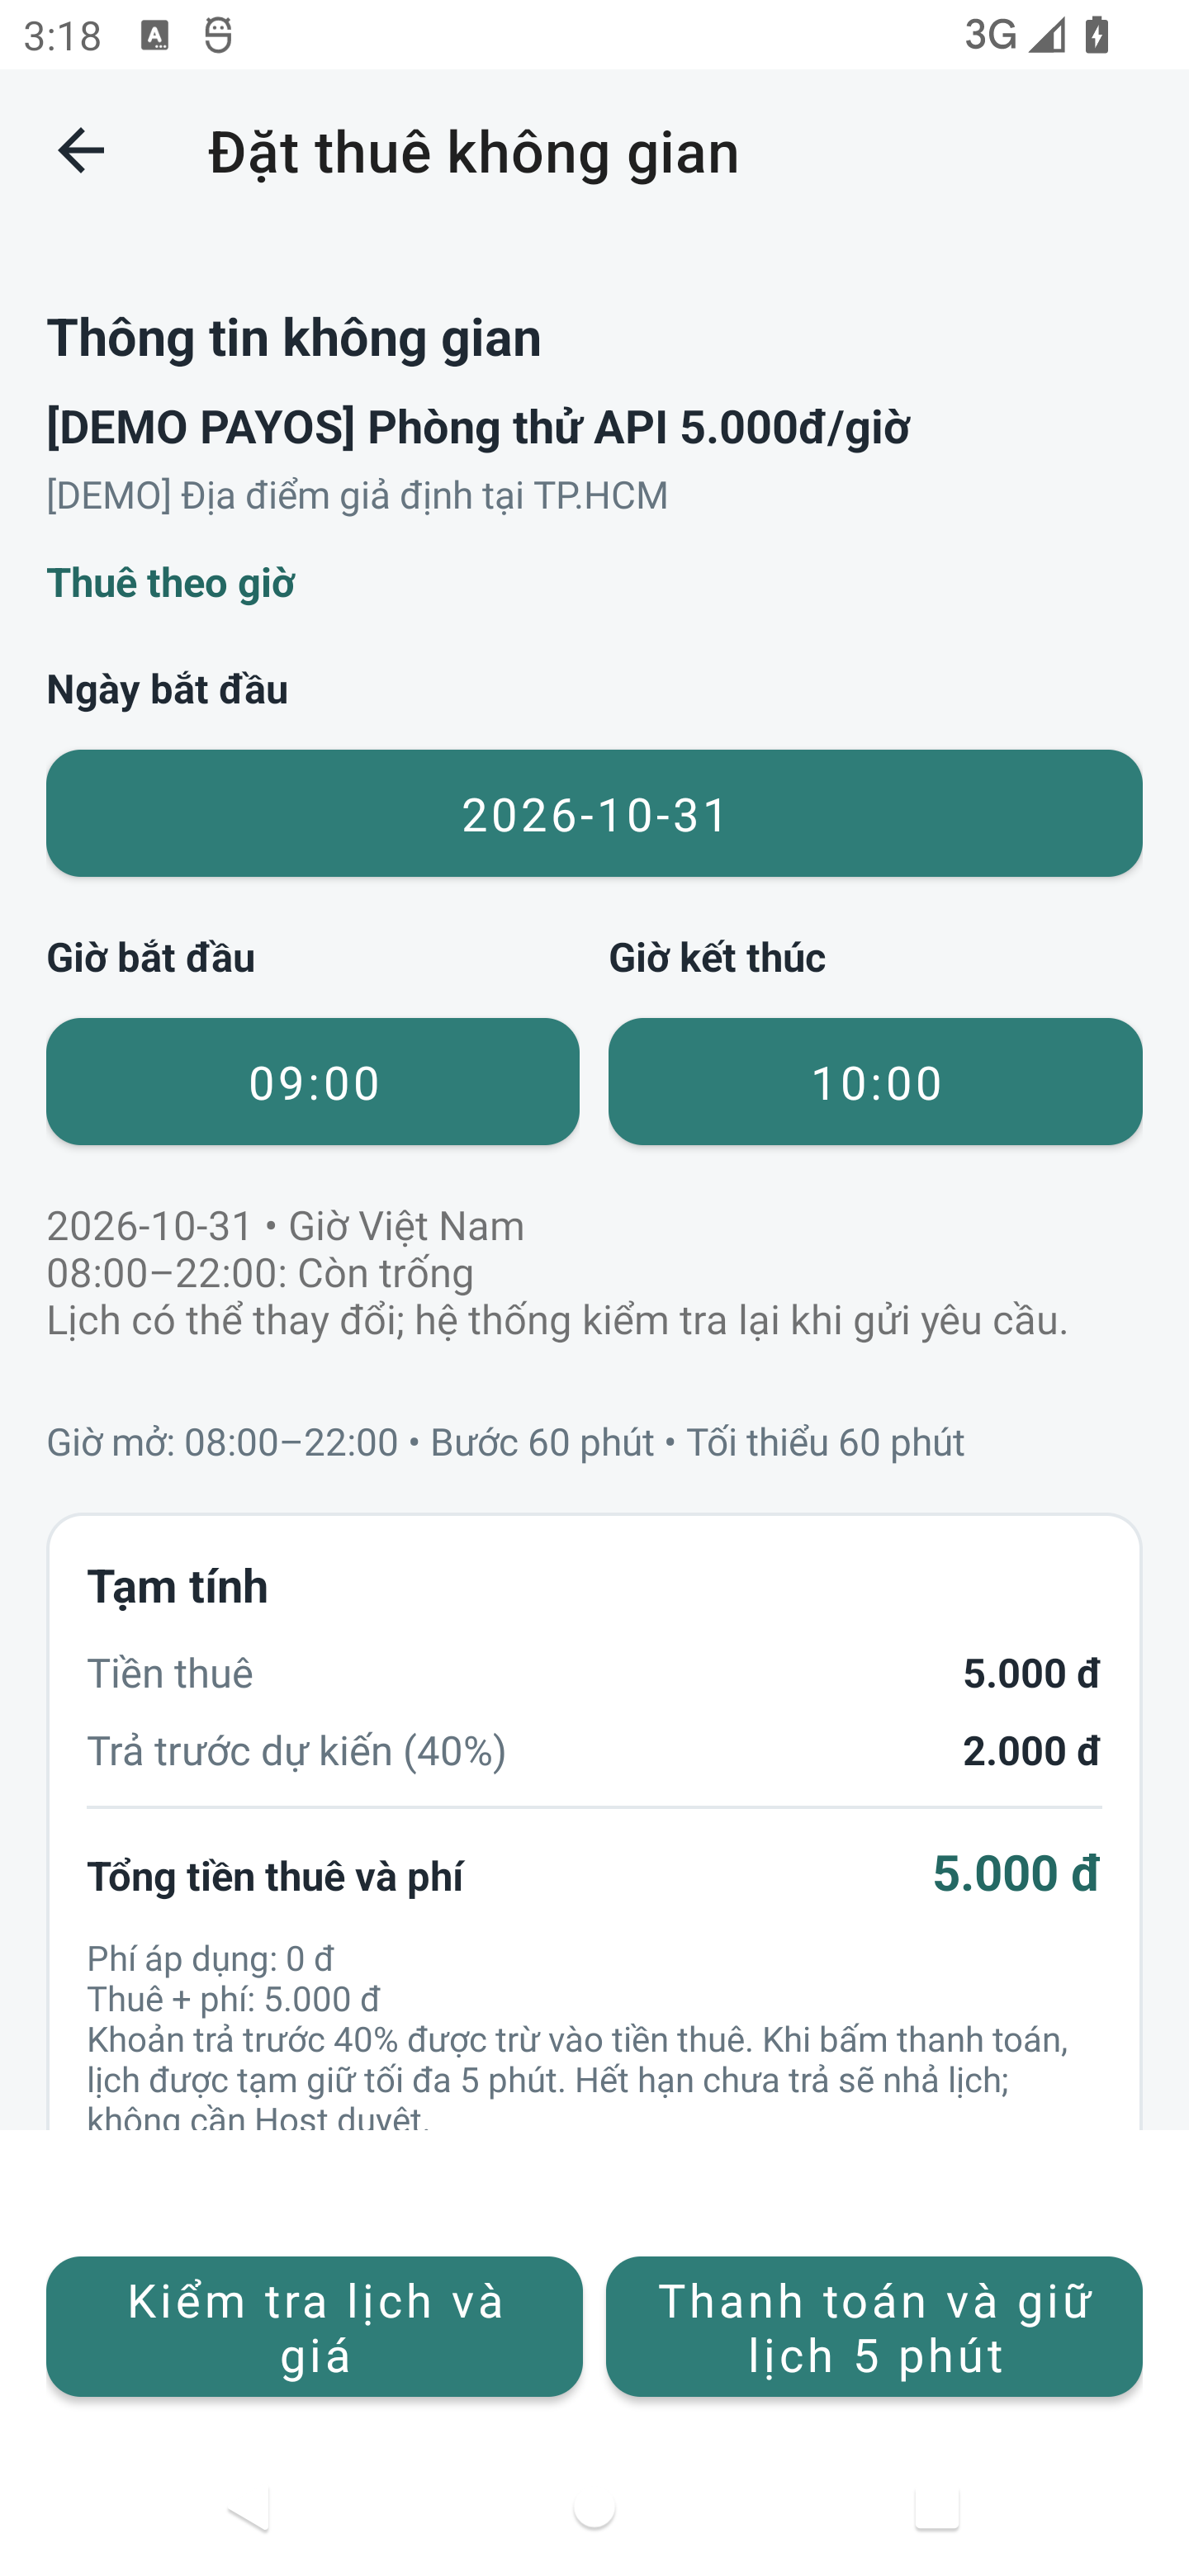
\includegraphics[width=\linewidth]{chapter6/booking-quote.png}\\[-1mm]
{\small (a) Kết quả kiểm tra lịch và giá}
\end{minipage}\hspace{0.05\linewidth}%
\begin{minipage}[t]{0.40\linewidth}\centering
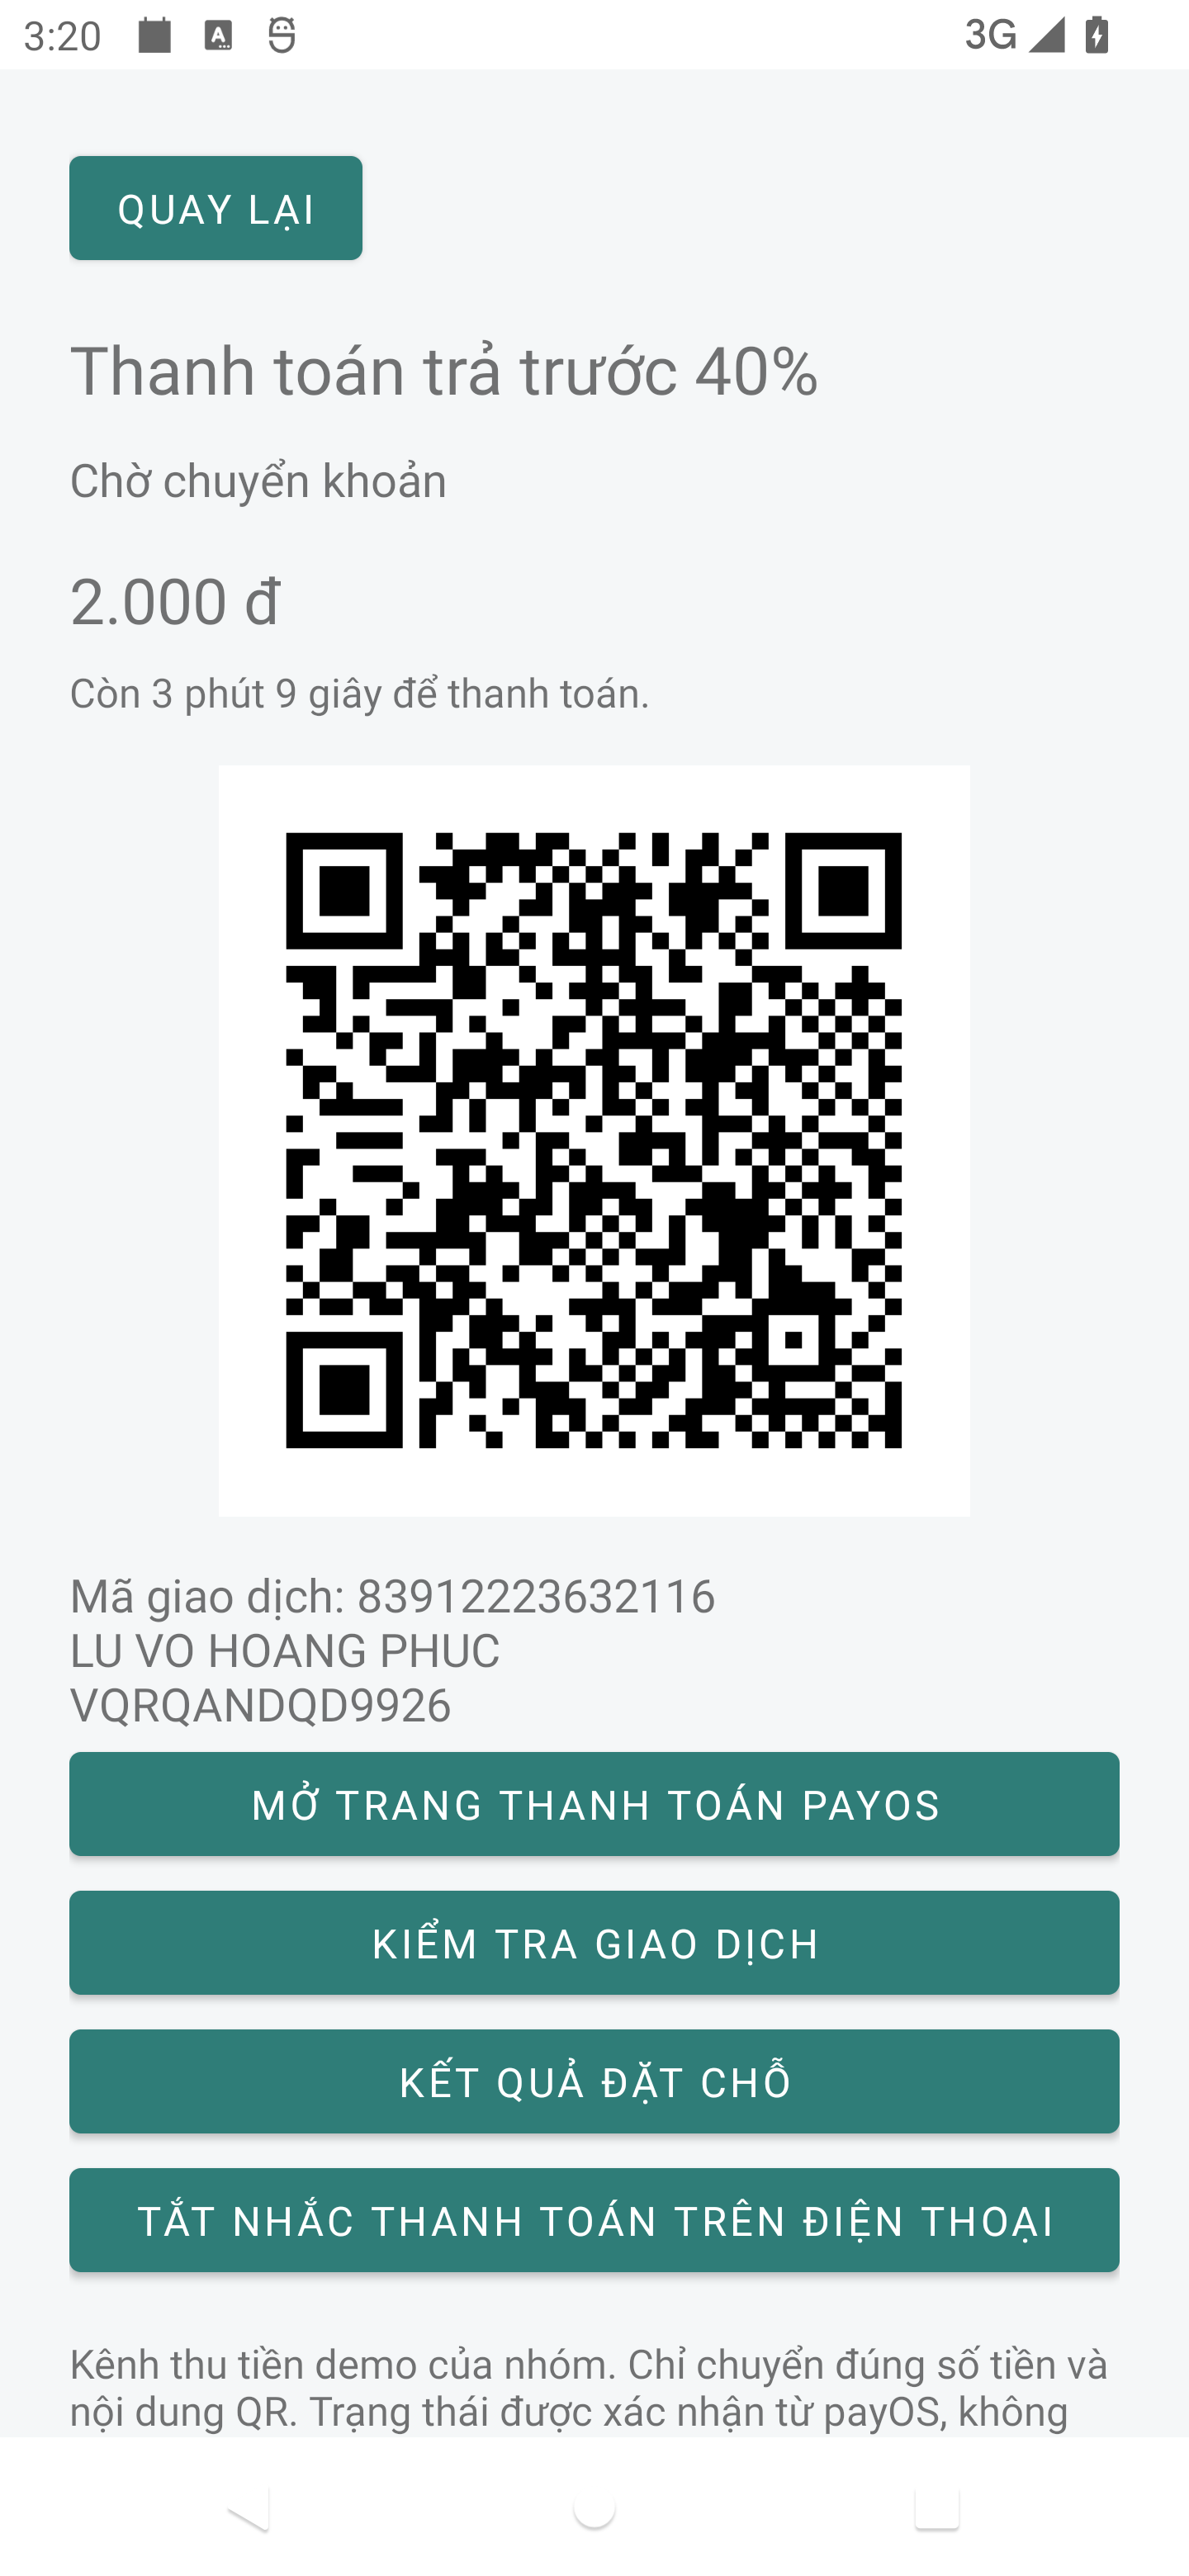
\includegraphics[width=\linewidth]{chapter6/booking-qr.png}\\[-1mm]
{\small (b) Phiên QR có thời hạn}
\end{minipage}
\caption{Từ kết quả kiểm tra lịch đến phiên thanh toán QR}
\label{fig:booking-quote-qr}
\end{minipage}
\end{figure}}{}

Khi payOS gửi dữ liệu thanh toán, webhook được chuyển tới backend BroomSharing để xác thực và đối soát. Backend kiểm tra giao dịch, số tiền và thời điểm thanh toán trước khi cập nhật trạng thái. Nhận đủ 40\% đúng hạn mới chuyển booking sang CONFIRMED và ghi nhận PAID; lịch đang giữ tiếp tục thuộc booking đó. Listener cập nhật kết quả trên Android, đồng thời thông báo thanh toán được đổi trạng thái. Booking không cần Host duyệt trước bước này.

\IfFileExists{Resources/chapter6/booking-paid.png}{%
\begin{figure}[H]
\begin{minipage}{\linewidth}
\setlength{\parindent}{1.27cm}
\setstretch{1.4}
Hình~\ref{fig:booking-payment-outcomes} ghi nhận hai kết quả ở hai giao dịch khác nhau. Ở Hình~\ref{fig:booking-payment-outcomes}(a), giao dịch đã nhận 2.000 đồng và booking được xác nhận. Ở Hình~\ref{fig:booking-payment-outcomes}(b), người thuê chưa trả tiền khi hết năm phút; backend khép booking EXPIRED, nhả lịch và ứng dụng hiển thị đặt chỗ không thành công. QR hết hạn được gỡ khỏi màn hình, thông báo điện thoại đổi sang kết quả thất bại. Nút xem kết quả đưa người thuê tới chi tiết booking để theo dõi trạng thái cuối.
\par\medskip
\centering
\begin{minipage}[t]{0.40\linewidth}\centering
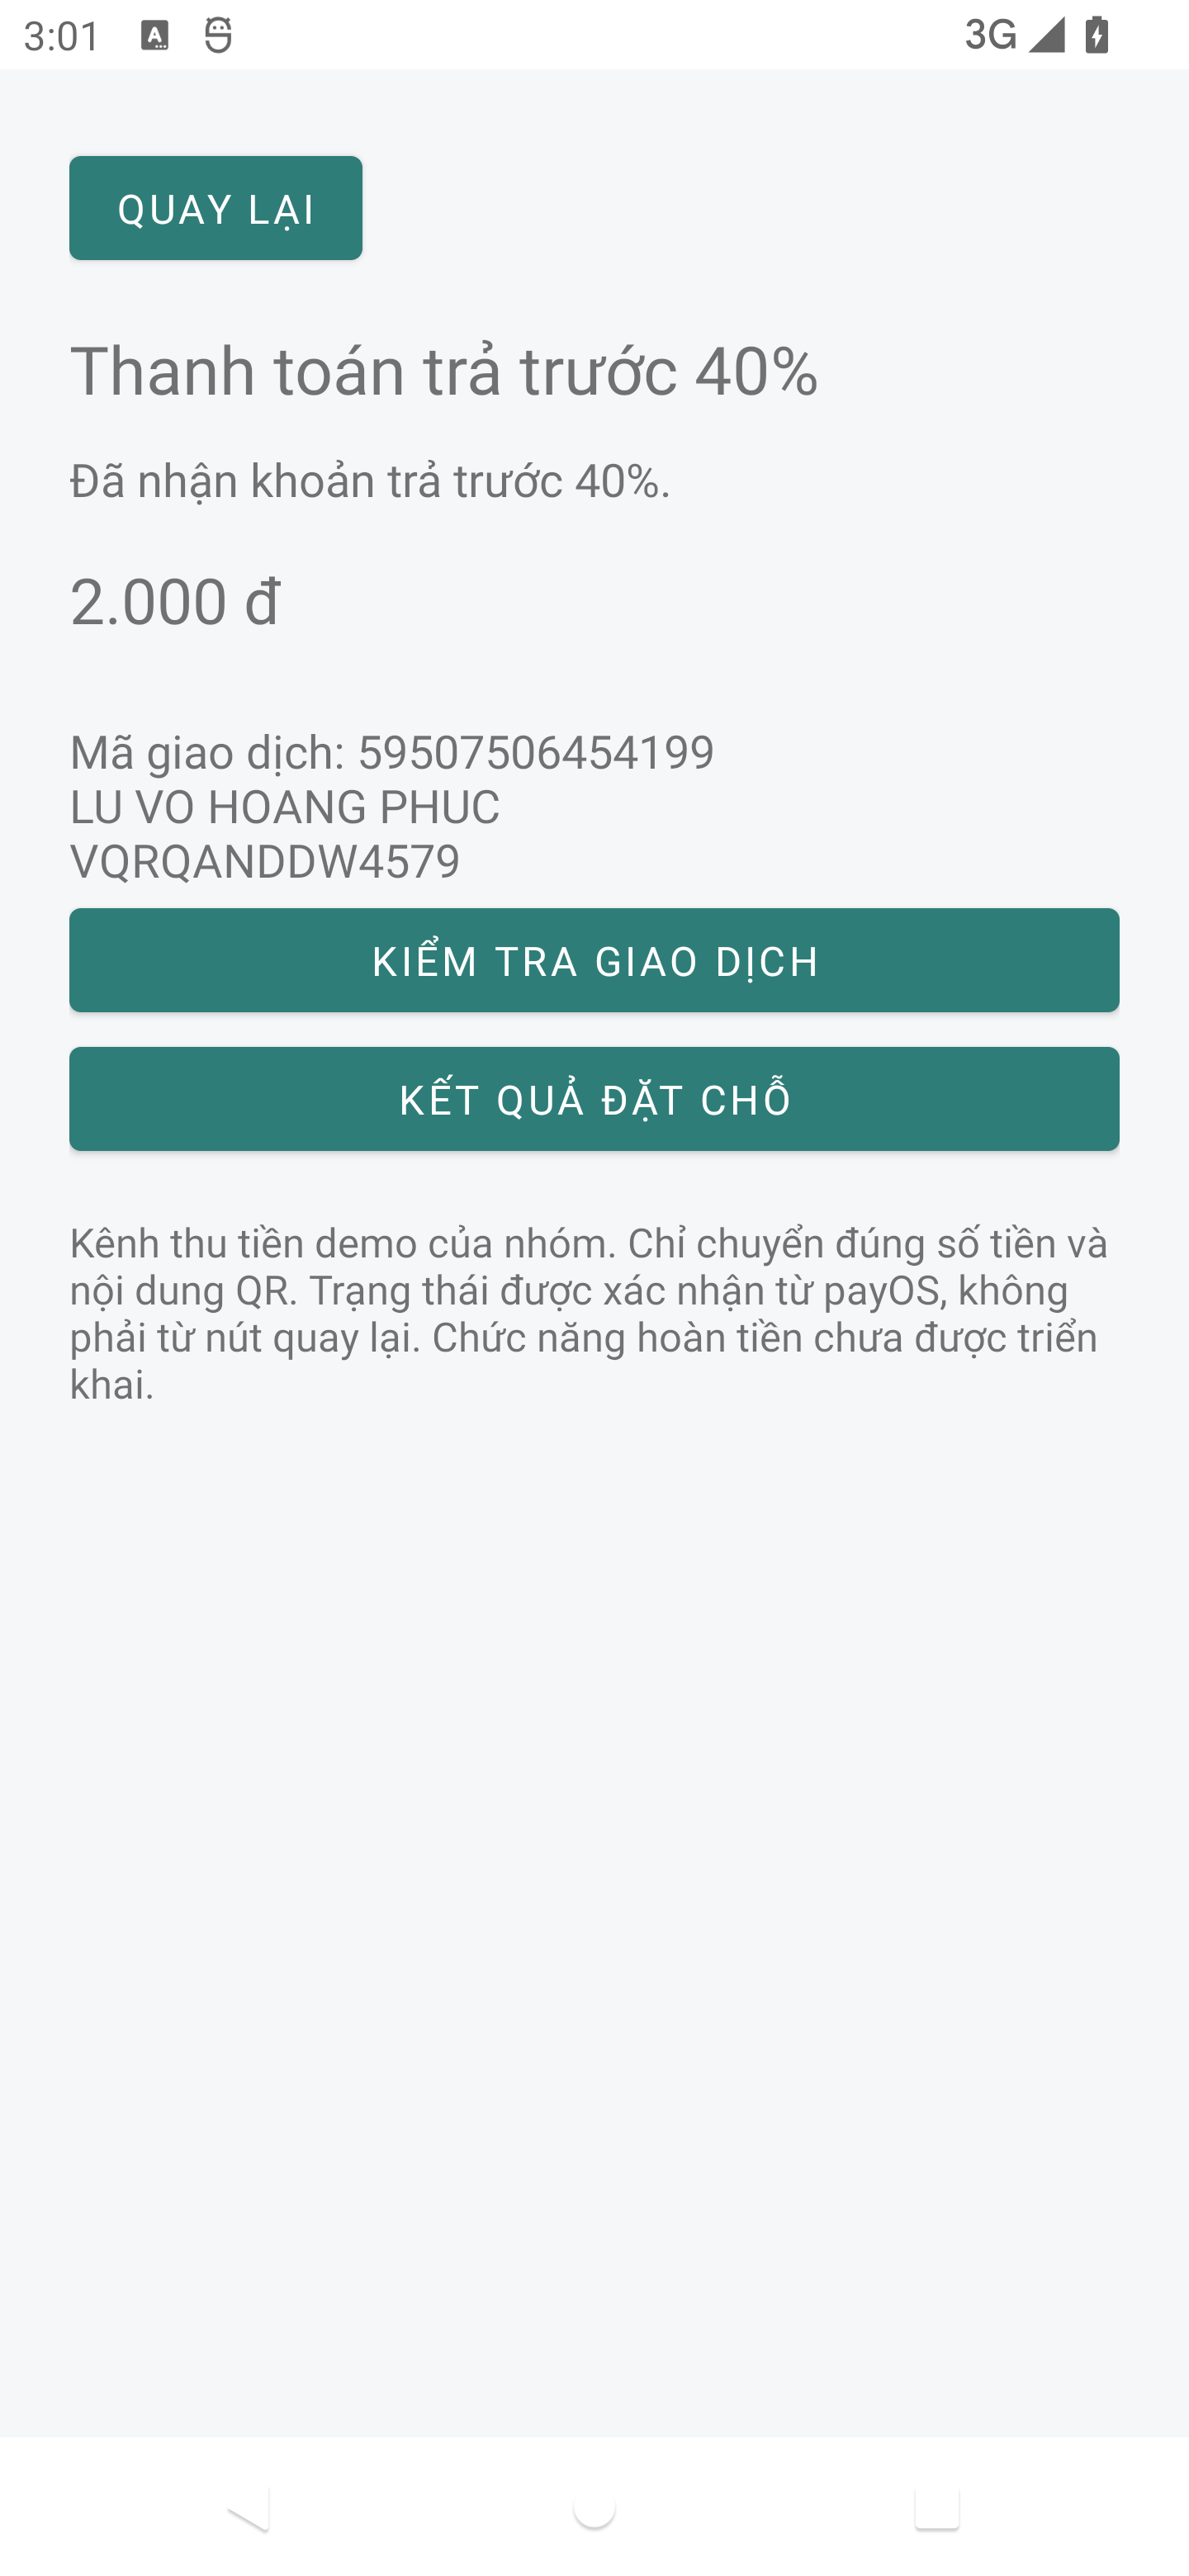
\includegraphics[width=\linewidth]{chapter6/booking-paid.png}\\[-1mm]
{\small (a) Đã ghi nhận thanh toán}
\end{minipage}\hspace{0.05\linewidth}%
\begin{minipage}[t]{0.40\linewidth}\centering
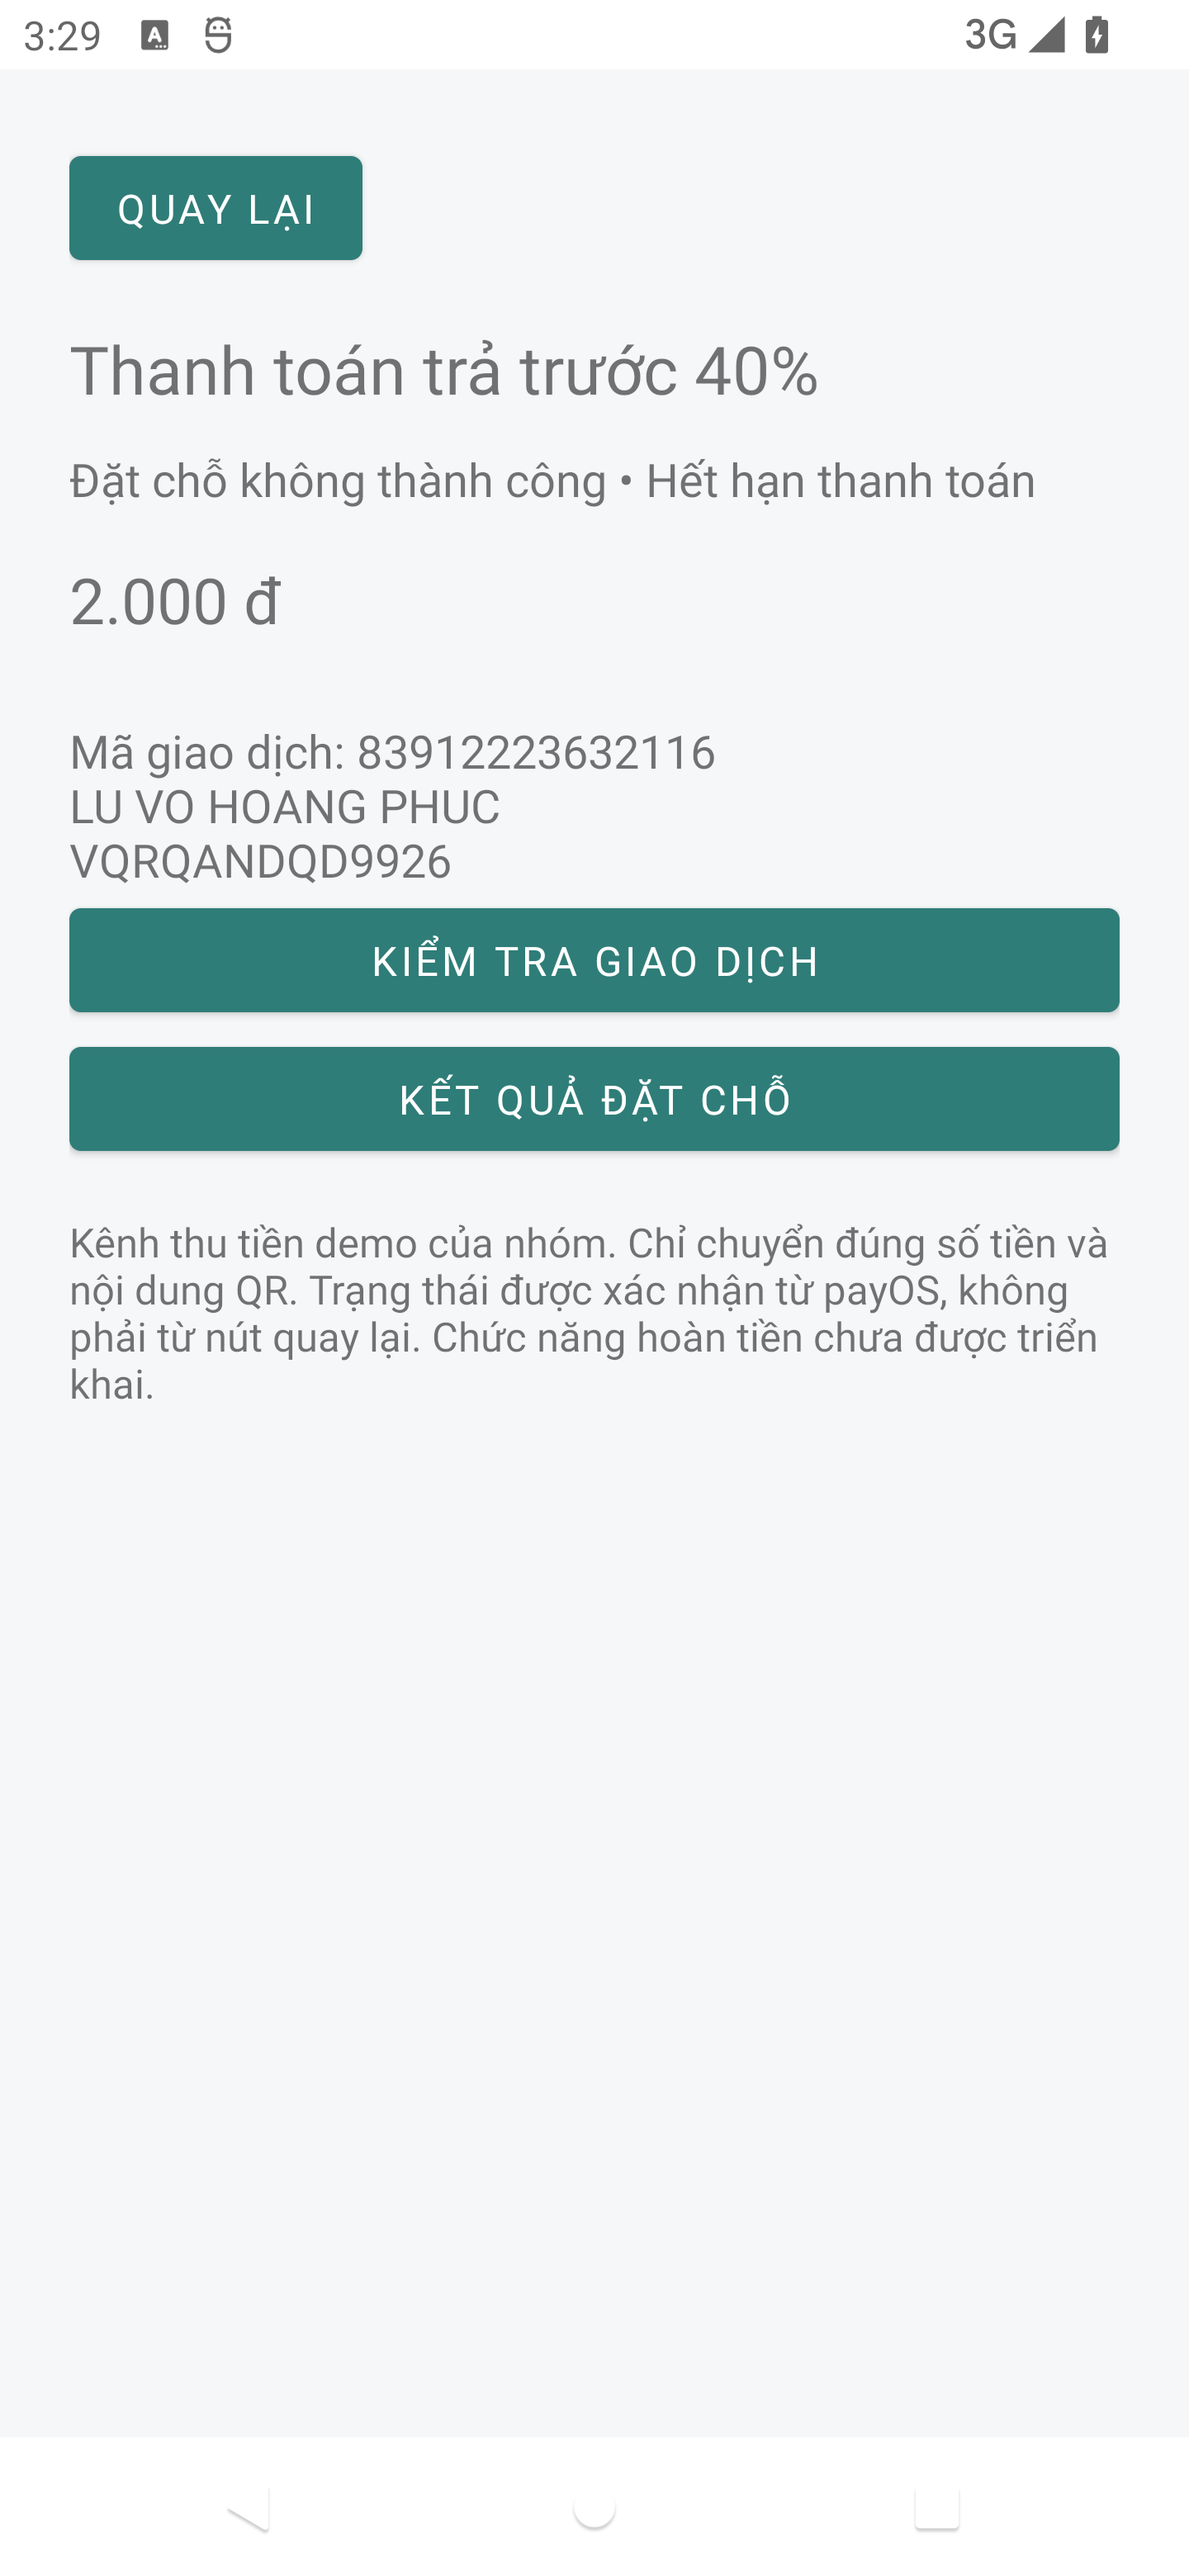
\includegraphics[width=\linewidth]{chapter6/booking-expired.png}\\[-1mm]
{\small (b) Hết hạn chưa thanh toán}
\end{minipage}
\caption{Kết quả xác nhận và hết hạn của các phiên đặt chỗ}
\label{fig:booking-payment-outcomes}
\end{minipage}
\end{figure}}{}

Người thuê theo dõi trạng thái cuối tại danh sách và chi tiết đặt chỗ. Trường hợp nhận tiền muộn hoặc dữ liệu tiền cần kiểm tra không được tự chuyển thành đã xác nhận; hệ thống giữ thông tin để đối soát thủ công. Phiên bản đồ án chưa thực hiện hoàn tiền qua API. Xác nhận thanh toán cũng không tự ghi khách đã đến hoặc đã sử dụng phòng; các mốc nhận phòng và hoàn tất thuộc quá trình thực hiện lượt thuê.

\clearpage
\noindent\begin{minipage}{\linewidth}
\captionsetup{hypcap=false}
\setstretch{1.4}
\noindent Hình~\ref{fig:booking-resume-notification}(a) cho thấy thẻ tiếp tục thanh toán khi một phiên còn hiệu lực. Người thuê chạm nút để mở lại đúng giao dịch với thời gian còn lại, thay vì chọn ngày và tạo booking mới. Thẻ chỉ xuất hiện khi có phiên đang chờ. Khi đã xác định hết hạn chưa trả tiền, thông báo điện thoại đổi sang đặt chỗ không thành công như Hình~\ref{fig:booking-resume-notification}(b); chạm thông báo mở kết quả liên quan. Bộ đếm tại thiết bị chỉ hỗ trợ hiển thị, còn kết quả tiền và việc nhả lịch do backend đối soát.
\par\medskip
\centering
\begin{minipage}[t]{0.40\linewidth}\centering
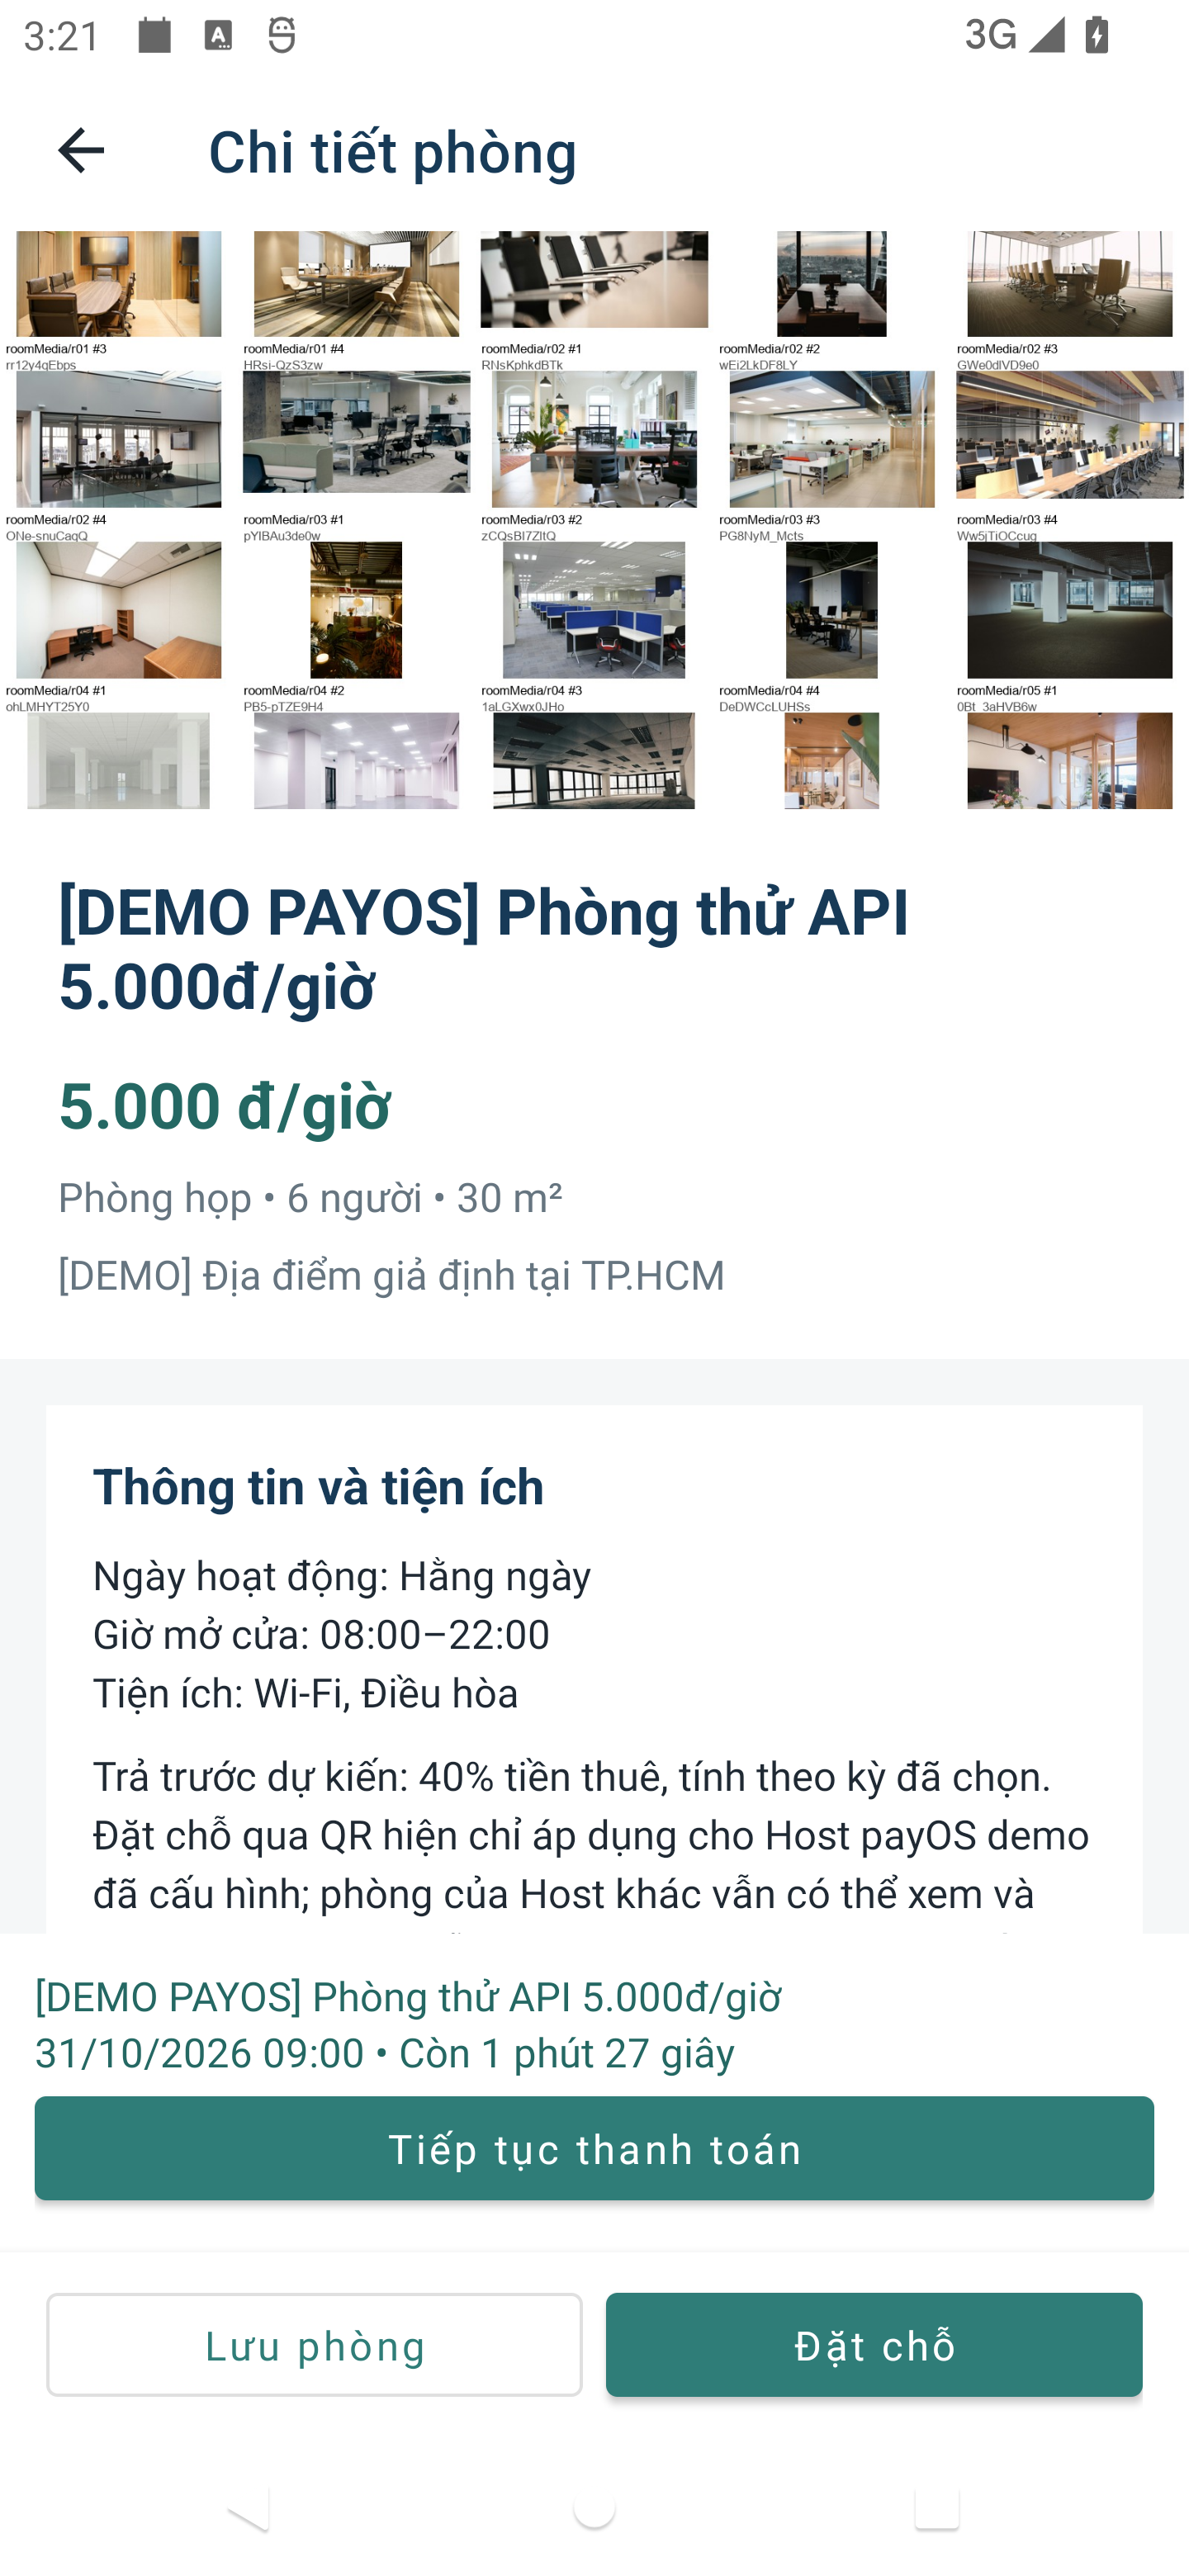
\includegraphics[width=\linewidth]{chapter6/booking-resume.png}\\[-1mm]
{\small (a) Tiếp tục phiên còn hạn}
\end{minipage}\hspace{0.05\linewidth}%
\begin{minipage}[t]{0.40\linewidth}\centering
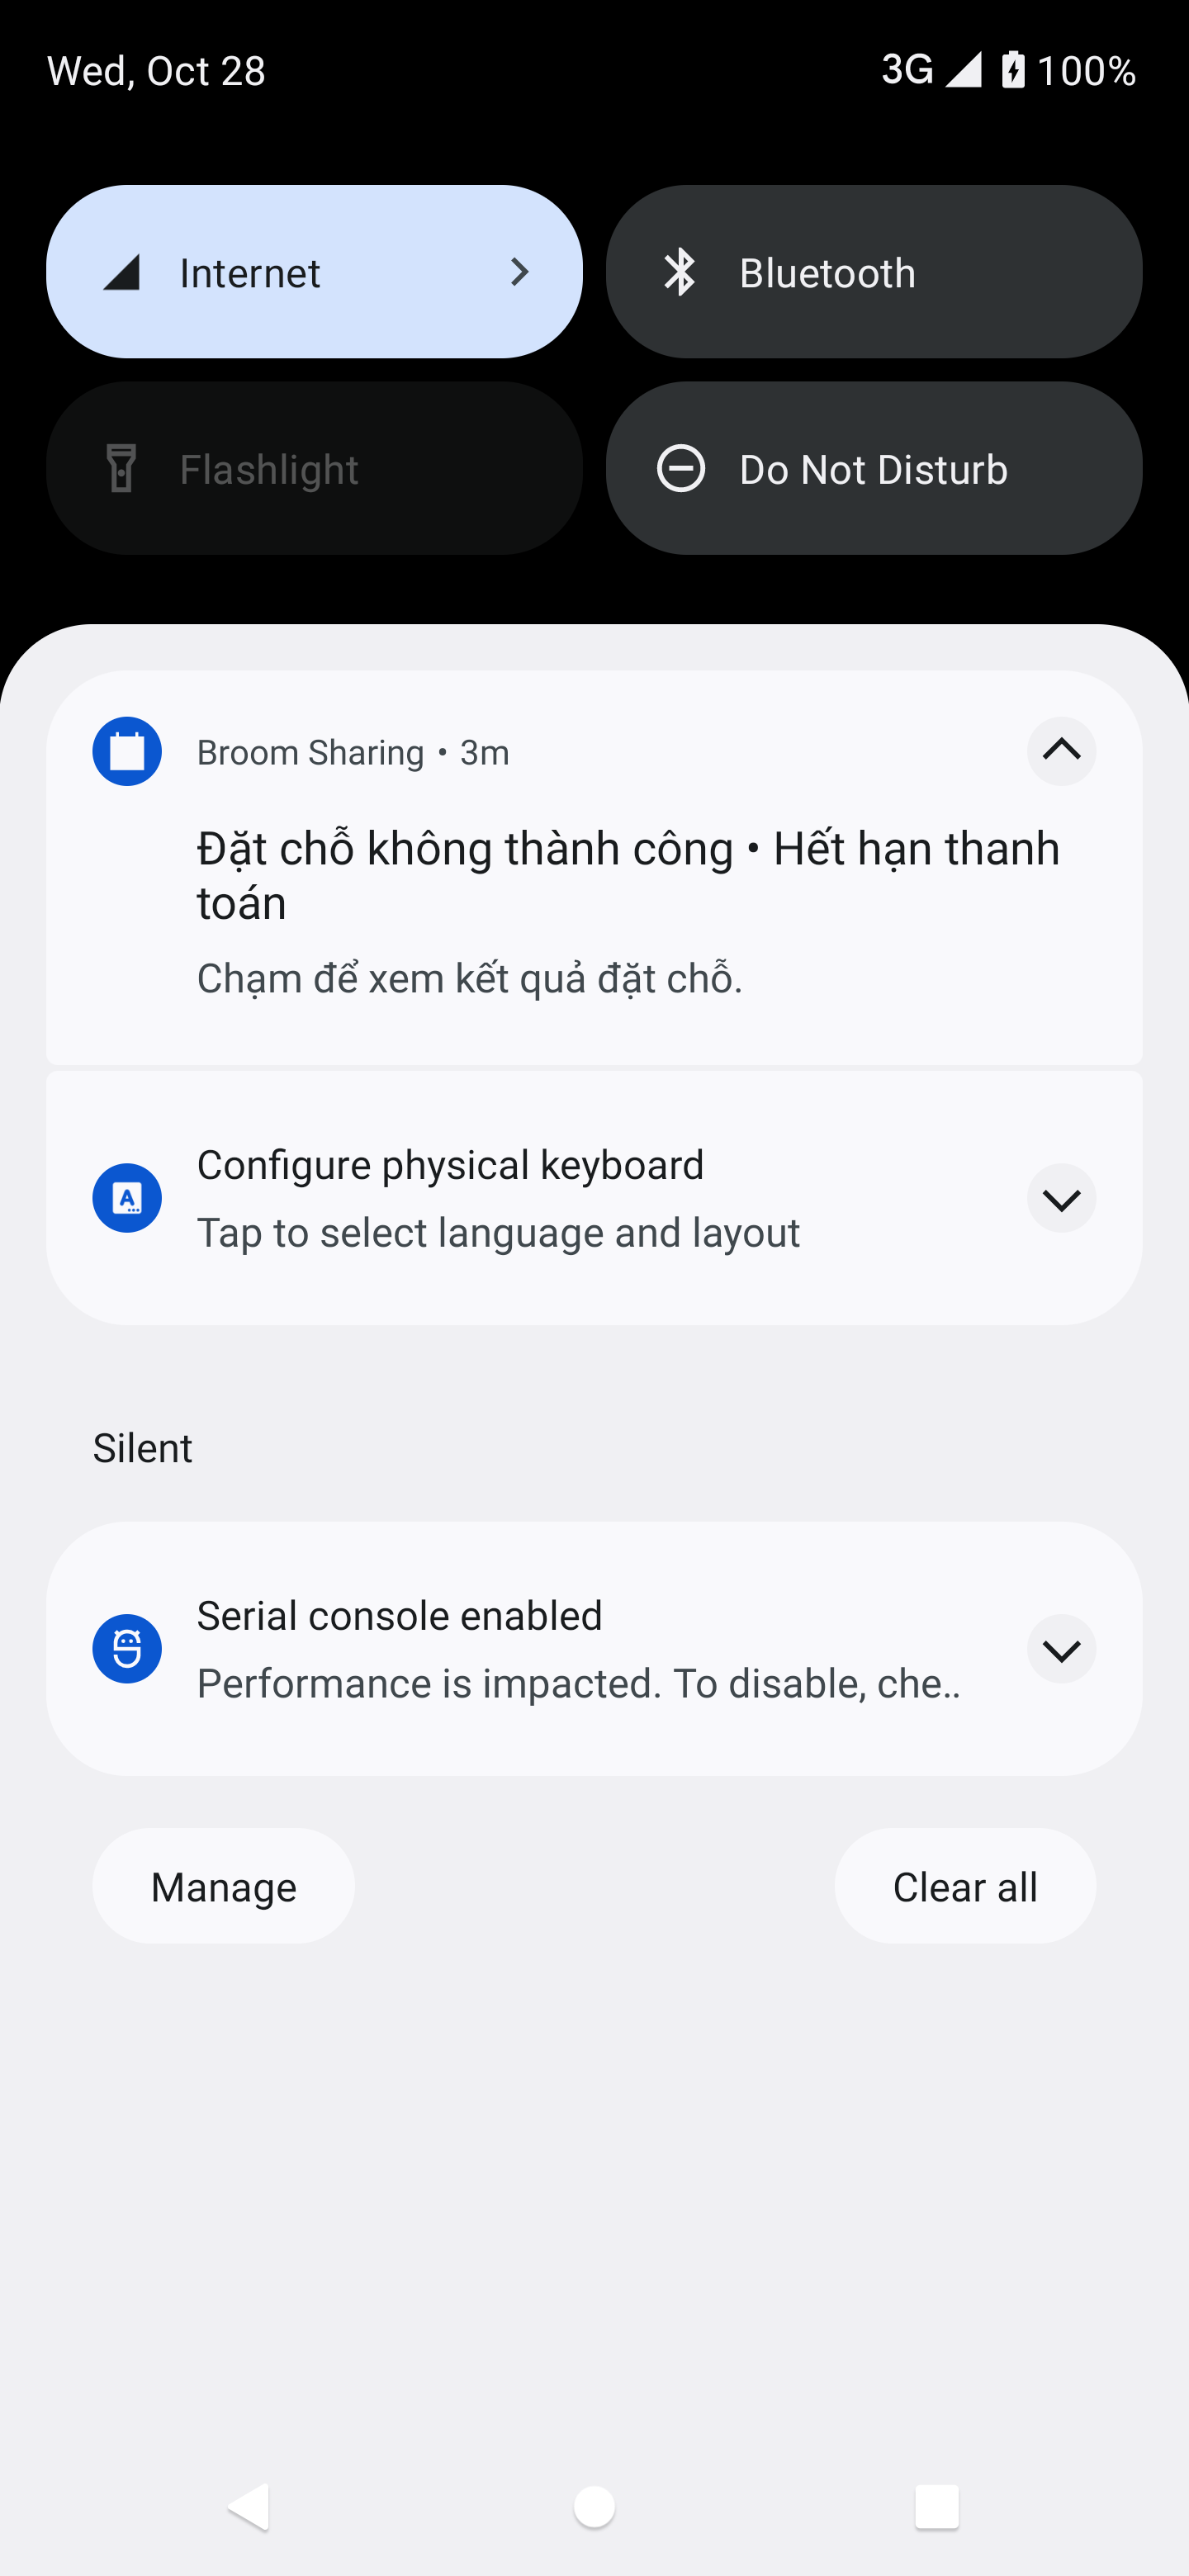
\includegraphics[width=\linewidth]{chapter6/booking-phone-notification.png}\\[-1mm]
{\small (b) Thông báo kết quả hết hạn}
\end{minipage}
\captionof{figure}{Tiếp tục giao dịch và nhận kết quả qua thông báo điện thoại}
\label{fig:booking-resume-notification}
\end{minipage}
\par
